\pagestyle{cyrill}
\section{Beobachterentwurf} \label{sec:beobachter}

Die Grund-Idee hinter dem Observer (Beobachter) ist, dass wenn innere Zustände des Systems nicht messtechnisch erfasst werden können, ein Modell des Systems „parallel“ mitläuft, aus dem dann die inneren Zustände bekannt sind und diese für eine Regelung genutzt werden können. Damit das Modell und das physikalische System nicht auseinander driften, werden die Abweichungen zwischen dem physikalischen Modell und dem Observer-Modell verglichen und dieser Fehler von einem Regler im Observer, der auf die inneren Zustände wirkt, zu null ausgeregelt. Das setzt zwei Dinge voraus:
\begin{itemize}
\item Das Modell des Observers muss hinreichend exakt sein, dass der Regelfehler nicht zu groß wird.
\item Der Regler des Observers muss schneller als der Regler sein, der auf die physikalische Strecke wirkt, da er in gewisser Weise einen inneren Regelkreis einer kaskadierten Reglerstruktur darstellt und sich die Regler sonst gegenseitig aufschwingen.
\end{itemize}

In diesem Projekt soll ein Luenberger-Beobachter verwendet werden. Die Matrix der Reglerkoeffizienten des Observers werden mit $L$ bezeichnet. Der Beobachter hat die in \autoref{fig:Bild8.1} gezeigte Struktur.

\begin{figure}[H]
   \centering
   \fbox{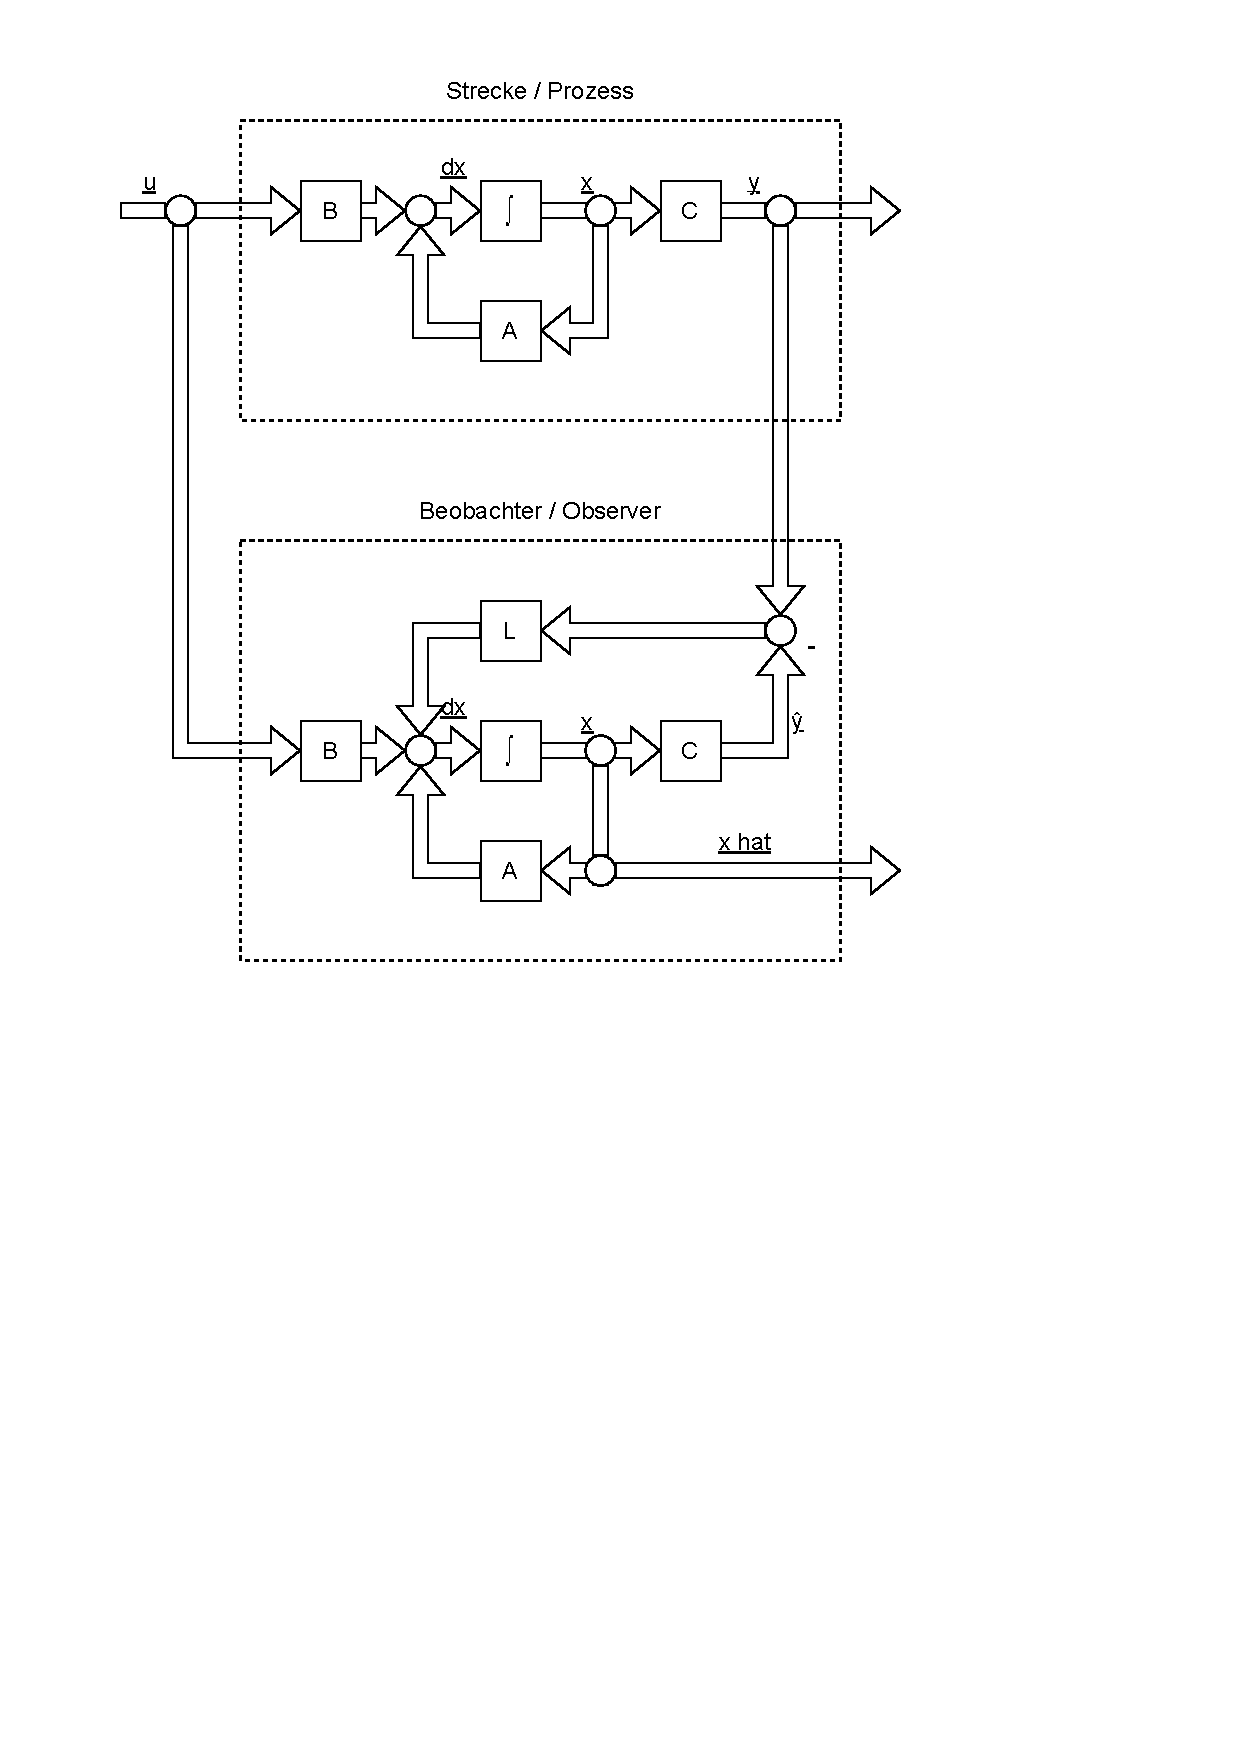
\includegraphics[width=0.95\textwidth]{Bilder/8_beobachterentwurf/Observer.pdf}}
   \caption[Beobachter-Reglerstruktur]{Struktur des Luenberger Beobachter}
   \label{fig:Bild8.1}
\end{figure}

Der Observer hat in unserem Fall zwei Eingänge und vier Ausgänge. Damit handelt es sich um ein MIMO (Multi-Input, Multi-Output) System. Dadurch ist ein Regler Entwurf nach Ackermann nicht mehr möglich.
Deshalb soll hier auf einen Regler Entwurf mittels LMI (vgl. \autoref{sec:LMI})  zurückgegriffen werden. Dabei werden keine konkreten Wunschpolstellen mehr vorgegeben, sondern ein Bereich, in dem die Polstellen liegen sollen. In unserem Fall soll dieser Bereich durch ein Alpha definiert sein, was gewisser Weise eine Schranke darstellt, hinter der die Polstellen liegen sollen.
Damit der Observer funktionieren kann, muss dieser steuerbar sein. Dies wird wieder, wie schon beim Ackermann-Regler-Entwurf mit der Steuerbarkeits-Matrix $Q_s$ überprüft. Diese berechnet sich in diesem Fall zu:

\begin{equation} \label{eq:Gleichung8.1}
    \underline{Q}_s = \begin{pmatrix} \underline{C}_{\mathrm{Obs}} \\ \underline{C}_{\mathrm{Obs}} \cdot \underline{A} \\ \cdots \\  \underline{C}_{\mathrm{Obs}} \cdot \underline{A}^{\mathrm{n-1}} \end{pmatrix}
\end{equation}

\begin{equation} \label{eq:Gleichung8.2}
    rank(\underline{Q}_s) = n
\end{equation}
\newline
Falls \autoref{eq:Gleichung8.2} gilt, ist der Observer steuerbar. Wobei $n$ hier die Anzahl der linear unabhängigen Spalten bezeichnet.

Anschließend werden wieder die Wunschpolstellen als ein Vielfaches (in unserem Fall dem zweifachen) der Polstellen des geschlossenen Regelkreises als Alphawerte ermittelt und als Alpha für den LMI-Entwurf verwendet. Das garantiert, dass die Polstellen des geschlossenen Regelkreises mit den ermittelten Regler Koeffizienten in dem Pol-Nullstellen-Diagramm links der Polstellen des Reglers der Strecke liegen.
Die Grundidee eines LMI-Entwurfs für den Regler wurde in \autoref{sec:LMI} bereits erläutert. Der Beobachter wird analog dazu entworfen, wobei statt einem System der Form $\dot{\underline{x}} = \underline{A} \cdot \underline{x}$ ein System der Form $\dot{\underline{x}} = \underline{A}\cdot \underline{x} \cdot \underline{B}\cdot (-\underline{k}\cdot \underline{x})$ eingesetzt (also für $\underline{u} = -\underline{k} \cdot \underline{x}$ eingesetzt), ergibt sich bei geforderte exponentiellen Stabilität eine nicht lineare Matrizen Ungleichung. Daher werden neue Variablen eingeführt mit $\underline{M} = \underline{k} \cdot \underline{X}$ und $\underline{P} = \underline{X}^{-1}$. Damit ergibt sich die LMI zu:

\begin{equation}
    \begin{split}
        \underline{0} &> \underline{X} \cdot \underline{A}^T + \underline{A} \cdot \underline{X} - \underline{M}^T \cdot \underline{B}^T - \underline{B} \cdot \underline{M} + 2 \cdot \alpha \cdot \underline{X}\\\\
        \underline{X} &> \underline{0}
    \end{split}
    \label{eq:Gleichung8.3}
\end{equation}
\newline

Damit ermittelt sich $\underline{k}$ zu $\underline{k} = \underline{M} \cdot \underline{X}^{-1}$.
Da das Modell des Beobachters die Form

\begin{equation}
    \begin{split}
        \underline{\dot{x}} &= \underline{A} \cdot \underline{e} - \underline{L} \cdot ( \underline{x} - \underline{\dot{\hat{x}}} )\\\\\underline{\dot{e}} &= \underline{\dot{x}} - \underline{\dot{\hat{x}}}
    \end{split}
    \label{eq:Gleichung8.4}
\end{equation}
hat, ergibt sich analog zum Regler Entwurf folgende LMI, wobei die neue Variable $\underline{N} = \underline{P} \cdot \underline{L}$ eingeführt wurde, wodurch sich $\underline{L}$ zu $\underline{L} = \underline{P}^{-1} \cdot \underline{N}$ ergibt:

\begin{equation}
    \begin{split}
        \underline{0} &> \underline{A}^T \cdot \underline{P} + \underline{P} \cdot \underline{A} - \underline{N} \cdot \underline{C} - \underline{C}^T \cdot \underline{N} + 2 \cdot \alpha \cdot \underline{P}\\\\
        \underline{P} &> \underline{0}
    \end{split}
    \label{eq:Gleichung8.5}
\end{equation}
\newline
Damit haben wir nun die LMI, die die Verstärkungsfaktoren unserer Rückführungs-Matrix beschreibt.
In \autoref{fig:Bild8.2} ist neben dem Aktuator-Eingang $u$ und dem Signal der Umschaltsteuerung die Abweichungsfehler des Beobachters für die vier internen Systemzustände zu sehen. Es ist deutlich zu erkennen, dass der Beobachter nur in der Nähe des Linearisierungs-Punktes zu gebrauchen ist (vgl. \autoref{sec:aufschwingen}).

\begin{figure}[H]
   \centering
   \fbox{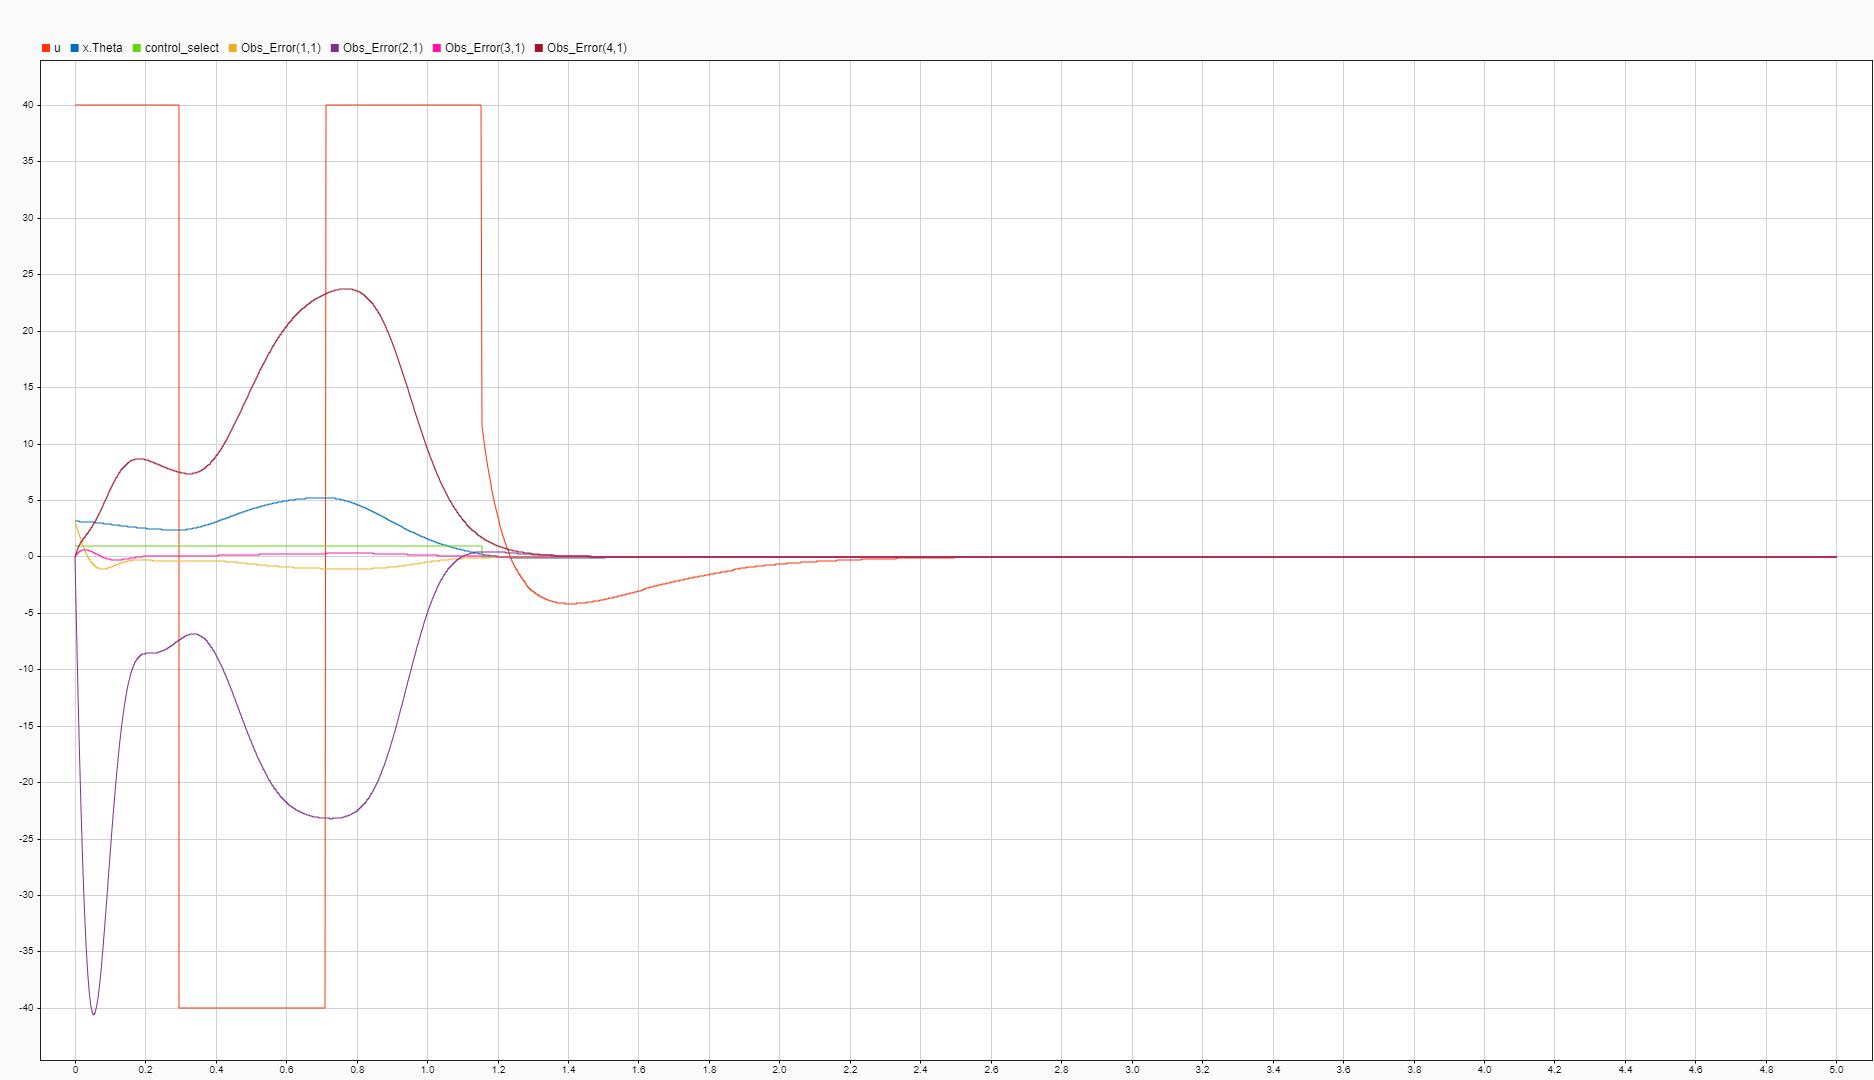
\includegraphics[width=0.95\textwidth]{Bilder/8_beobachterentwurf/Error_Beobachter2.png}}
   \caption[Beobachter-Abweichung]{Fehler des Luenberger Beobachter}
   \label{fig:Bild8.2}
\end{figure}